%%%%%%%%%%%%%%%%%%%%%%%%%%%%%%%%%%%%%%%%%%%%%%%%%%%%%%%%%%%%%%%%%%
\section{Simulación de las topologías en \acrshort{den2ne}}

Esta Sección viene dada por el objetivo de obtener el conjunto de datos final sobre el que se basará el desarrollo en el Capítulo \ref{cha:desarrollo}. Para lograrlo, se requiere llevar a cabo un gran número de  simulaciones en \gls{den2ne} a partir de las topologías generadas con la herramienta \gls{brite} (ver Sección \ref{sec:ejebrite}). 

\vspace{3mm}

No obstante, previamente a la ejecución del algoritmo, es imprescindible implementar una serie de modificaciones en el mismo para ajustar su funcionamiento para obtener resultados de utilidad para el presente \gls{tfm}. La secuencia de acciones que se llevará a cabo se detallará en la Sección \ref{sec:cambiosden2ne}. De la misma forma, se justificará el criterio escogido para determinar cúando se producen errores en el proceso de distribución energética. Esto servirá de base para después entrenar los modelos de \gls{ml} y \gls{dl}.

\vspace{3mm}

Por consiguiente, se añade la Sección \ref{sec:confden2ne}, donde se especificará la configuración de los parámetros de entrada de \gls{den2ne} y se cuantificará el número total de pruebas posibles que se podrían llegar a realizar a partir de las topologías generadas y de los datos reales procesados anteriormente. Se comprobará a través de diferentes pruebas que las modificaciones introducidas en el algoritmo \gls{den2ne} producen una operativa acorde a las necesidades de este \gls{tfm}. De forma concluyente, a partir de los resultados obtenidos en las simulaciones, se añadirá la Sección \ref{sec:datasetfinal}, en referencia a las características del dataset final que se utilizará para el entrenamiento de los modelos.

\subsection{Adaptación del algoritmo \acrshort{den2ne} a las pruebas}
\label{sec:cambiosden2ne}

Todas las modificaciones realizadas en el funcionamiento del algoritmo \acrshort{den2ne} han sido aplicadas a partir de los ficheros contenidos en el repositorio\footnote{https://github.com/NETSERV-UAH/den2ne-Alg} del equipo de investigación NetIS de la \gls{uah}.

\subsubsection{Importación de los perfiles de carga reales}
\label{sec:importcarga}

La primera modificación que se debe implementar en el funcionamiento de \gls{den2ne} consiste en la importación de los valores de carga reales, obtenidos como resultado de llevar a cabo la fase de procesamiento de los datos (ver Sección \ref{sec:combinacion}). La necesidad de aplicar este paso se debe a que el algoritmo, a partir de una topología dada a la entrada, establece una función de densidad de probabilidad para determinar de forma aleatoria un valor de carga para cada uno de los nodos de una topología. Para modificar este proceso se sigue la siguiente secuencia de pasos:

\begin{enumerate}
    \item Definición de función \textit{getLoads\_Config} en \textit{dataCollector.py}: Se añade una función de recolección de las configuraciones de carga reales, pasando como argumentos el directorio definido en \textit{path\_simtests} y el fichero de pruebas \textit{sim\_file}. Después, se inicializa una variable de diccionario y se almacenan los valores de potencia generada, consumida y la diferencia calculada de ambas. Estos valores se manejan en términos de kW, puesto que \gls{den2ne} está configurado para trabajar en esta unidad.
    \item Definición de funciones \textit{cargas} y \textit{cargas\_con\_limite} en \textit{brite\_intf.py}: Ambas funciones se encargan de aplicar los valores de carga reales, extraídos de la función anterior, a cada uno de los nodos de una topología determinada. En el caso de las simulaciones que se realizan en este \gls{tfm}, se hará uso de la primera, debido a que no se configuran límites de los valores de carga (ver Sección \ref{sec:confden2ne}). Por tanto, poniendo el foco en la función \textit{cargas}, se pasa como argumento el diccionario resultante de la función \textit{getLoads\_Config} y se extrae a partir de las claves del mismo el número de perfiles de carga (23) a manejar. De la misma forma, se pasa también como argumento el fichero de nodos, anteriormente generado con \gls{brite} y el \textit{parser}, para conocer las dimensiones que tiene la topología en cuestión. Con este dato se determina la cantidad de iteraciones que son necesarias para aplicar el valor de carga real a todos los nodos de una topología y, para cada uno de ellos, se determina de forma aleatoria uno de los 23 perfiles reales de carga. A la salida, se obtiene un nuevo diccionario con tamaño igual al número de nodos que hay en la topología y que viene constituido por la información del identificador del perfil real seleccionado y del valor de carga neta aplicada.
    \item Definición de la variable \textit{id\_orig} en \textit{node.py}: Se añade al constructor de la clase de nodo que tiene \gls{den2ne} un nuevo elemento, en relación al identificador del perfil de carga seleccionado para un nodo en cuestión.
    \item Introducción de la variable \textit{id\_orig} en la función \textit{buildGraph} en \textit{graph.py}: La nueva variable de nodo se incluye en el proceso de generación del grafo para mantener el conocimiento del perfil de carga que se ha seleccionado para cada nodo durante la ejecución completa del algoritmo.
    \item Modificaciones en \textit{test\_topo.py}: El fichero dedicado a las pruebas de \gls{den2ne} debe incluir las llamadas a las funciones creadas o modificadas anteriormente. También, requiere definir los nuevos parámetros \textit{path\_simtests} y \textit{sim\_file}, en referencia a los ficheros de prueba que contienen los valores de carga, extraídos del dataset para un instante temporal determinado (ver Sección \ref{sec:datasetfinal}).
\end{enumerate} 

\subsubsection{Introducción de la etiqueta de error}
\label{sec:etierror}
Como se había introducido en el Capítulo \ref{ch:intro}, el objetivo de este \gls{tfm} viene dado por la necesidad de poder detectar y predecir los errores que se pueden producir durante el proceso de distribución energética que realiza \gls{den2ne}. Por ello, una vez que se aplican los pasos anteriores, se debe definir el criterio de error a partir del cual se van a etiquetar los resultados extraídos del algoritmo. Teniendo en cuenta que para las simulaciones se configura un escenario real con pérdidas y limitación de capacidad de los enlaces (ver Sección \ref{sec:confden2ne}), se toma la decisión de establecer la condición de fallo en base a la existencia de un exceso de capacidad en un intercambio energético entre dos nodos:

\begin{enumerate}
    \item Introducción de la variable \textit{link\_overflow} en la función \textit{globalBalance} en \textit{den2neALG.py}: Para cada intercambio energético que se realiza en el proceso de distribución, se comprueba que la carga direccionada desde el nodo de origen al nodo destino no sobrepasa la capacidad del enlace que los interconecta. En caso afirmativo, se activa la variable \textit{link\_overflow} y, por el contrario, se deja con valor nulo, indicando que el intercambio se ha producido sin fallos. 
    \item Modificación de la función \textit{getLosses} en \textit{link.py}: \gls{den2ne}, en su funcionamiento original, calcula las pérdidas del enlace a partir del valor de carga intercambiado o de la propia capacidad, en función de sobrepasarla o no. A modo de depuración y de simplificar su funcionamiento, se incluye como argumento la etiqueta \textit{link\_overflow} y se modifica la estructura de la función.
\end{enumerate} 

\subsubsection{Extracción de resultados}
Para extraer de la ejecución del algoritmo unos resultados que contengan toda la información útil sobre la que se pueda crear el dataset final, es preciso aplicar las siguientes modificaciones:

\begin{enumerate}
    \item Definición de la función \textit{getLinkDist} en \textit{graph.py}: Se incluye una función para obtener la distancia existente entre el nodo de origen y de destino.    
    \item Introducción de la variable \textit{data\_topo} en la función \textit{globalBalance} en \textit{den2neALG.py}: Se define el diccionario \textit{data\_topo} y, para cada intercambio energético, se almacena en el mismo la información del nodo origen y destino (etiquetas jerárquicas y longitudes de las mismas), los datos del enlace (distancia y capacidad), el valor de la etiqueta de error y la carga que se intercambia. En el caso de las longitudes de las etiquetas jerárquicas, se añaden las líneas de código necesarias en \textit{globalBalance} para extraer las mismas.
    Modificaciones en \textit{test\_topo.py}: Se cambia la llamada a la función \textit{globalBalance} para poder extraer el diccionario \textit{data\_topo} de la misma. También, se establece la nomenclatura que tendrán los ficheros de resultados. Como se expondrá más adelante en la Sección \ref{sec:datasetfinal}, esta nomenclatura se determina en base a la información dada por el instante temporal del fichero de test y por el resto de parámetros configurados en el script de automatización de pruebas \textit{auto\_run.sh}.
    \item Modificaciones en \textit{auto\_run.sh}: Se añaden los parámetros que hacen referencia al directorio donde se ubican los ficheros de test y a cada uno de los mismos para automatizar las pruebas (ver Sección \ref{sec:datasetfinal}).
\end{enumerate} 

\subsubsection{Configuración de la capacidad de los enlaces}
Como paso adicional, se modifican las capacidades de los enlaces que se proporcionan por defecto en el fichero \textit{links\_config.csv}. Esto se realiza con el objetivo de que el algoritmo configure enlaces de menor capacidad con la misma probabilidad que los de mayor, puesto que este proceso es aleatorio. A modo de simplificación, se establecen los tres tipos de enlaces definidos en la Tabla \ref{tab:links}

\vspace{3mm}

\begin{table}[h!]
    \centering
    \begin{tabular}{|c|c|c|}
    \hline
    \rowcolor[HTML]{AAAAAA}
    \multicolumn{1}{|c|}{\cellcolor[HTML]{AAAAAA}\textit{R (ohm/km)}} & \multicolumn{1}{c|}{\cellcolor[HTML]{AAAAAA}\textit{I max (A)}} & \textit{Sección (mm²)} \\ \hline
    0,272 & 185 & 70 \\ \hline
    0,78 & 100 & 25 \\ \hline
    1,91 & 53 & 10 \\ \hline
    \end{tabular}
    \caption{Configuraciones de enlaces de \textit{links\_config.csv}}
    \label{tab:links}
\end{table}

\subsection{Configuración de los parámetros de entrada}
\label{sec:confden2ne}

Para ejecutar \gls{den2ne}, es preciso definir la configuración de los parámetros de entrada en el script \textit{auto\_run.sh}. Este script se diseña con el objetivo de automatizar las simulaciones en el algoritmo y, como se ha expuesto en la Sección \ref{sec:cambiosden2ne}, ha sido necesario ajustar el mismo a los requerimientos de las pruebas de este \gls{tfm}. El cálculo de la cantidad total de simulaciones que se pueden ejecutar en \gls{den2ne} viene dado por el producto de todas los parámetros siguientes:

\begin{itemize}
    \item El número total de topologías generadas: En la Sección \ref{sec:gentopo} se especifica una cantidad total de 180 topologías obtenidas a la salida de la herramienta \gls{brite}.
    \item El número de instantes temporales del dataset: El conjunto de datos resultante de la etapa de procesamiento, detallado en la Sección \ref{sec:combinacion} y, específicamente, en la Tabla \ref{tab:datacombinacion}, abarca una cantidad de filas igual al total de instantes temporales que se han tomado en consideración. En otros términos, al tratarse de muestras tomadas cada hora durante un rango temporal que comprende un año completo, su valor se calcula como 24x365=8760 instantes.
    \item El número de criterios: Como se detallaba en la Sección \ref{sec:den2ne}, \gls{den2ne} presenta 6 criterios de selección de los mejores caminos hacia el nodo raíz. En este caso, se implementan a las pruebas los 6 tipos.
    \item El número de tipos de escenarios de red: En la Sección \ref{sec:den2ne}, también se exponían los 4 tipos de escenarios que permite configurar el algoritmo. Teniendo en cuenta que las simulaciones deben acercarse a un entorno de \gls{sg} real y que el objetivo se basa en encontrar las transacciones energéticas entre nodos que superen la capacidad del enlace, se determina únicamente el escenario de pérdidas y límite de capacidad.
    \item Modo de limitación de carga: Se especifica únicamente el modo que determina valores de carga ilimitados.
    \item El número de semillas de ejecución: De la misma manera que se ha especificado anteriormente para \gls{brite} (ver Sección \ref{sec:conftopo}), se aplica al algoritmo \gls{den2ne} un conjunto de archivos de semillas para obtener simulaciones diferentes a partir de una misma topología a la entrada. En este caso, debido a la cantidad de datos que ya se maneja y para no introducir latencias considerables en el lanzamiento de las pruebas, se especifican 5 semillas por topología.
\end{itemize}

Por otro lado, en el caso de los parámetros de entrada referentes a las topologías, como son el número de nodos por topología, los modelos a simular y el número de semillas de generación, se sigue la misma configuración especificada en la ejecución de \gls{brite} (ver Sección \ref{sec:conftopo}). No obstante, para el grado de conectividad se determinan directamente los valores reales, suponiendo enlaces bidireccionales.

\vspace{3mm}

\begin{lstlisting}[language=bash, style=Consola, caption={Configuración de los parámetros de entrada en el script de automatización de \acrshort{den2ne}}]
TOPO_CRITERIONS=(0 1 2 3 4 5) # Criterios de selección de IDs
TOPO_BEHAVIORAL=3 # Tipo de escenario de red = modo Losses and Capacity (3)         
TOPO_LOAD_LIMIT=0 # Sin limite de carga
TOPO_RUNS=5 # Seeds de ejecución de DEN2NE

TOPO_NAMES=('barabasi' 'waxman') # Empleo de modelos RTWaxman y RTBarabasi (igual que BRITE)
TOPO_NUM_NODES=$(seq 100 50 200) # Número de nodos por topología (igual que BRITE)
TOPO_DEGREES=(2 4 6) # El grado de conectividad real (en BRITE 1, 2, 3)
TOPO_SEEDS=(1 2 3 4 5 6 7 8 9 10) # Seeds de generación de BRITE
\end{lstlisting}

\vspace{3mm}

Por tanto, teniendo en cuenta la configuración implementada para los parámetros de entrada, se puede determinar el número total de simulaciones únicas posibles a partir de la siguiente expresión:

    \[\textit{Nsim} = \textit{Ntopos} \times \textit{Ninstantes} \times \textit{Ncriterios} 
    \times \textit{Nescenarios} \times \textit{NNlimit} \times \textit{Nsem\_ejec}\]
    \[\textit{Nsim} = 180 \times 8760 \times 6 \times 1 \times 1 \times 5 = 47304000\] 

\pagebreak 

\subsection{Creación del dataset final y conclusiones de las pruebas}
\label{sec:datasetfinal}

Teniendo en cuenta el número total de simulaciones únicas posibles calculado en la Sección \ref{sec:confden2ne}, se debe decidir qué pruebas se van a realizar en el algoritmo para construir el dataset final, puesto que es ineficiente e inviable ejecutar todas las posibilidades. Por lo tanto, se opta por escoger 12 instantes temporales, haciendo referencia a una hora determinada de un día por cada mes. 

\vspace{3mm}

Por simplificar, como el rango temporal de las muestras (ver Sección \ref{sec:rango}) comienza el 28 de noviembre de 2010, se decide seleccionar los días 28 de cada mes. De la misma forma, para la hora se escogen las 11:00, ya que este es el momento del día en el que se aprecia una mayor producción energética de media (ver Figura \ref{fig:average}). En consecuencia, en los resultados de la ejecución de \gls{den2ne} se obtendrá un mayor número de intercambios energéticos con fallos, al existir una mayor probabilidad de exceder la capacidad de los enlaces. Esta selección es importante para conseguir un dataset final sobre el que se pueda entrenar de una forma correcta los modelos del Capítulo \ref{cha:desarrollo}. No obstante, previamente a detallar la secuencia de acciones realizadas para construir este conjunto de datos final, se debe introducir el diagrama de la Figura \ref{fig:total2} para aportar una mayor comprensión de esta Sección. 

\begin{figure}[H]
    \centering
    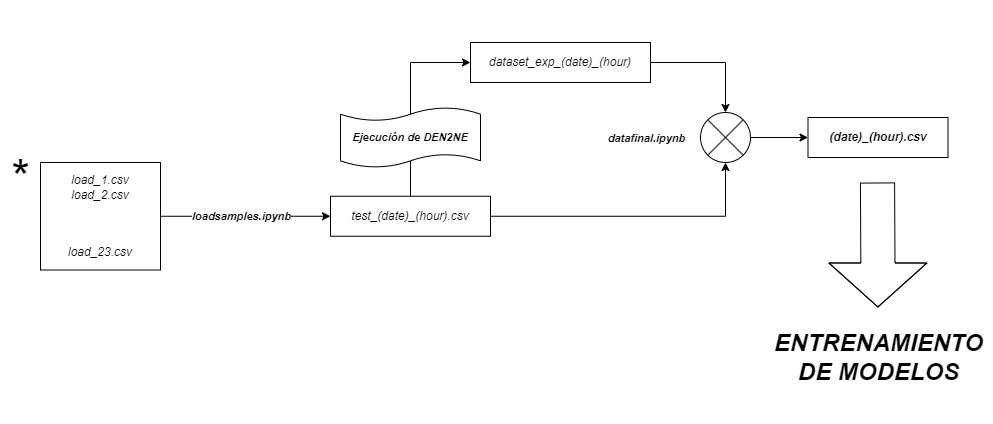
\includegraphics[width=1\textwidth]{img/diseno/total2.png}
    \caption{Diagrama completo de diseño del dataset final}
    \label{fig:total2}
\end{figure}

\vspace{3mm}

Como el objetivo se basa en extraer de los ficheros finales de cargas netas \textit{load\_x.csv} (ver Sección \ref{sec:combinacion}) los datos de los instantes temporales especificados, se introduce un nuevo \textit{notebook}, denominado como \textit{loadsamples.ipynb}. A partir del mismo, se filtran los 12 instantes seleccionados y se obtienen a la salida 12 ficheros de test (ej. \textit{test\_2010-11-28\_11.csv}), los cuales serán proporcionados a la entrada del algoritmo para importar los 23 perfiles reales de carga para cada prueba. Es en este paso cuando se proceden a ejecutar las simulaciones en \gls{den2ne}. La aplicación de cada fichero de test a la entrada proporciona a la salida un nuevo directorio nombrado con el instante temporal que especifica el fichero de test en cuestión (ej. \textit{dataset\_exp\_2010-11-28\_11}). En su interior, se impone una organización de los resultados en 18 carpetas, en función del modelo y del grado de conectividad al que hacen referencia (ej. \textit{barabasi\-200\-6}). Cada una de dichas carpetas consta de 60 ficheros de resultados, que incluyen en su nombre el número de semilla, el criterio del algoritmo, el instante temporal, el grado de conectividad y el modelo (ej. \textit{dataset\_seed\_1\_cr\_0\_t\_2010\-11\-28\_11\_dg\_2\_m\_barabasi.csv}). En la Figura \ref{fig:dirnombres} se expone la nomenclatura especificada para cada uno de los directorios y ficheros de resultados.

\vspace{3mm}

\begin{figure}[h!]
    \centering
    \begin{minipage}{0.4\textwidth}
      \centering
      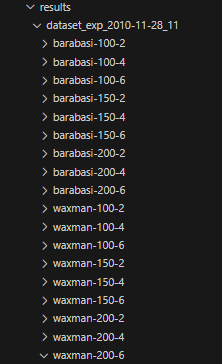
\includegraphics[width=\linewidth]{img/diseno/dirpruebas2.png}
      \label{fig:dirpruebas2}
    \end{minipage}\hfill
    \begin{minipage}{0.6\textwidth}
      \centering
      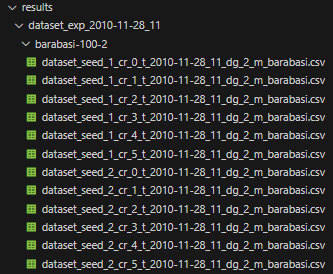
\includegraphics[width=\linewidth]{img/diseno/dirpruebas.png}
      \label{fig:dirpruebas}
    \end{minipage}\hfill
    \caption{Nomenclatura de los directorios y ficheros de resultados}
    \label{fig:dirnombres}
\end{figure}

\vspace{3mm}

Por lo tanto, se puede expresar que para cada prueba ejecutada o fichero de test a la entrada de \gls{den2ne}, se obtienen a la salida un total de 1080 ficheros de resultados. Cada uno de ellos presenta un número de filas igual a la cantidad de nodos de la topología simulada, o expresado de otra forma, igual al total de intercambios energéticos realizados (100, 150 o 200 filas). Con esto, ya es posible crear el dataset final mediante un nuevo \textit{notebook}, denominado como \textit{datafinal.ipynb}. A modo de simplificar el tratamiento de los resultados del algoritmo, se agrupa primero, en un mismo \textit{dataframe} el contenido de los 1080 ficheros resultantes de cada prueba. 

\vspace{3mm}

Después, se comprueba que el porcentaje total de intercambios erróneos o con exceso de capacidad de enlace no es nulo para la prueba en cuestión. Es decir, si no se obtiene ninguna fila con la etiqueta \textit{link\_overflow} activa, no se podrán predecir errores cuando se desarrollen y se entrenen los modelos y, por ello, se debería utilizar otro instante temporal para las simulaciones. 

\vspace{3mm}

Una vez realizada esta comprobación, la siguiente acción se basa en combinar los ficheros de resultados con el resto de medidas que proporcionan los ficheros de test. Las filas de ambos se agrupan a partir del perfil de carga configurado en el nodo origen, especificado por el valor del identificador real. Tras esta operación, el nuevo \textit{dataframe} en \textit{datafinal.ipynb} se constituye por todas las columnas de datos. En este paso es importante revisar y eliminar aquellas que están replicadas, como ocurre en el caso del identificador y la fecha. 

\vspace{3mm}

\begin{lstlisting}[style=Python, caption={Combinación de ficheros de resultados y de test}]
    df_merged = pd.merge(df, df_sim, left_on='origen_id', right_on='iid', how='outer')
\end{lstlisting}

\vspace{3mm}

Finalmente, se almacena el \textit{dataframe} ya limpio en un fichero, cuyo nombre hace referencia al instante temporal de la prueba en cuestión (ej. \textit{2010-12-28\_11.csv}). Este fichero contiene un total de 160920 filas con un valor de etiqueta de error y con toda la información respectiva a cada intercambio energético simulado. Por ello, se define como el conjunto de datos final resultante de una prueba o instante temporal determinado. Como se han ejecutado 12 pruebas, si se agrupan los 12 conjuntos finales, se puede calcular una cantidad total de 1931040 intercambios etiquetados sobre los que entrenar los modelos. De forma adicional, se añade la Tabla \ref{tab:datafinal} para exponer los campos que contienen cada uno de los conjuntos finales.

\vspace{3mm}

Con la obtención de estos 12 ficheros finaliza la etapa de diseño y, por ende, el presente Capítulo. A partir de los resultados obtenidos, se puede expresar de forma concluyente que se cumple el objetivo principal de generar un dataset completo, sobre el cual se entrenarán y desarrollarán los modelos en el Capítulo \ref{cha:desarrollo}. 

\begin{table}[h!]
    \centering
    \begin{tabular}{|c|c|c|}
    \hline
    \rowcolor[HTML]{AAAAAA} 
    \multicolumn{1}{|c|}{\cellcolor[HTML]{AAAAAA}Campo} & \multicolumn{1}{c|}{\cellcolor[HTML]{AAAAAA}Descripción} & Unidades \\ \hline
    \textit{timestamp} & Instante temporal de medida & datetime \\ \hline
    \textit{datetime} & Fecha del valor promedio & datetime \\ \hline
    \textit{H} & Hora del valor promedio & - \\ \hline
    \textit{overflow} & Etiqueta binaria de superación de carga & - \\ \hline
    \textit{cap} & Capacidad del enlace & kW \\ \hline
    \textit{load} & Carga neta (\textit{Dif}) & kW \\ \hline
    \textit{dist} & Distancia & m \\ \hline
    \textit{origen\_id} & Identificador de nodo origen & - \\ \hline
    \textit{dest\_id} & Identificador de nodo destino & - \\ \hline
    \textit{len\_origen\_tag} & Longitud de la etiqueta del nodo origen & - \\ \hline
    \textit{len\_dest\_tag} & Longitud de la etiqueta del nodo destino & - \\ \hline
    \textit{modelo} & Modelo de topología & - \\ \hline
    \textit{criterion} & Criterio de selección de IDs & - \\ \hline
    \textit{degree} & Grado de conectividad & - \\ \hline
    \textit{total\_balance} & Balance de carga global & - \\ \hline
    \textit{abs\_flux} & Flujo total de carga en el nodo raíz & - \\ \hline
    \textit{Diffuse Irradiance} & Índice de radiación difusa (\gls{dif}) & W/m2 \\ \hline
    \textit{Plane of Array Irradiance} & Índice de radiación en el plano del array (\acrshort{poa}) & W/m2 \\ \hline 
    \textit{Ambient Temperature} & Temperatura ambiente & C \\ \hline
    \textit{Cell Temperature} & Temperatura de las células solares & C \\ \hline
    \textit{DC Array Output} & Potencia de salida DC del array & W \\ \hline
    \textit{AC System Output} & Potencia de salida AC del sistema & W \\ \hline
    \textit{Pavg} & Potencia consumida & W \\ \hline
    \textit{Dif} & Carga neta calculada & W \\ \hline
    \end{tabular}  
    \caption{Dataset final obtenido por cada instante temporal probado en \acrshort{den2ne}}
    \label{tab:datafinal}
\end{table}


